%----------------------------------------------------------------------------
\chapter{Overview of the Approach}
%----------------------------------------------------------------------------
In this chapter, the various aspects of the proposed approach are detailed. In Section \ref{sec_methodology}, the application of this methodology from the users' point of view: how are they supposed to interact with the interactive automata learning framework and how can they utilize it to design reactive systems declaratively. Then, in Section \ref{sec_architecture}, the applied software architecture, software components, algorithms and data structures are presented in the following order: first, the components concerned with the automata learning algorithm, then those responsible for its interaction with the oracle, then the possible interactions of the oracle with the engineer.
%----------------------------------------------------------------------------
\section{Overview of the Methodology} \label{sec_methodology}
%----------------------------------------------------------------------------
\begin{figure}[!ht] 
	\centering
	\fbox{
		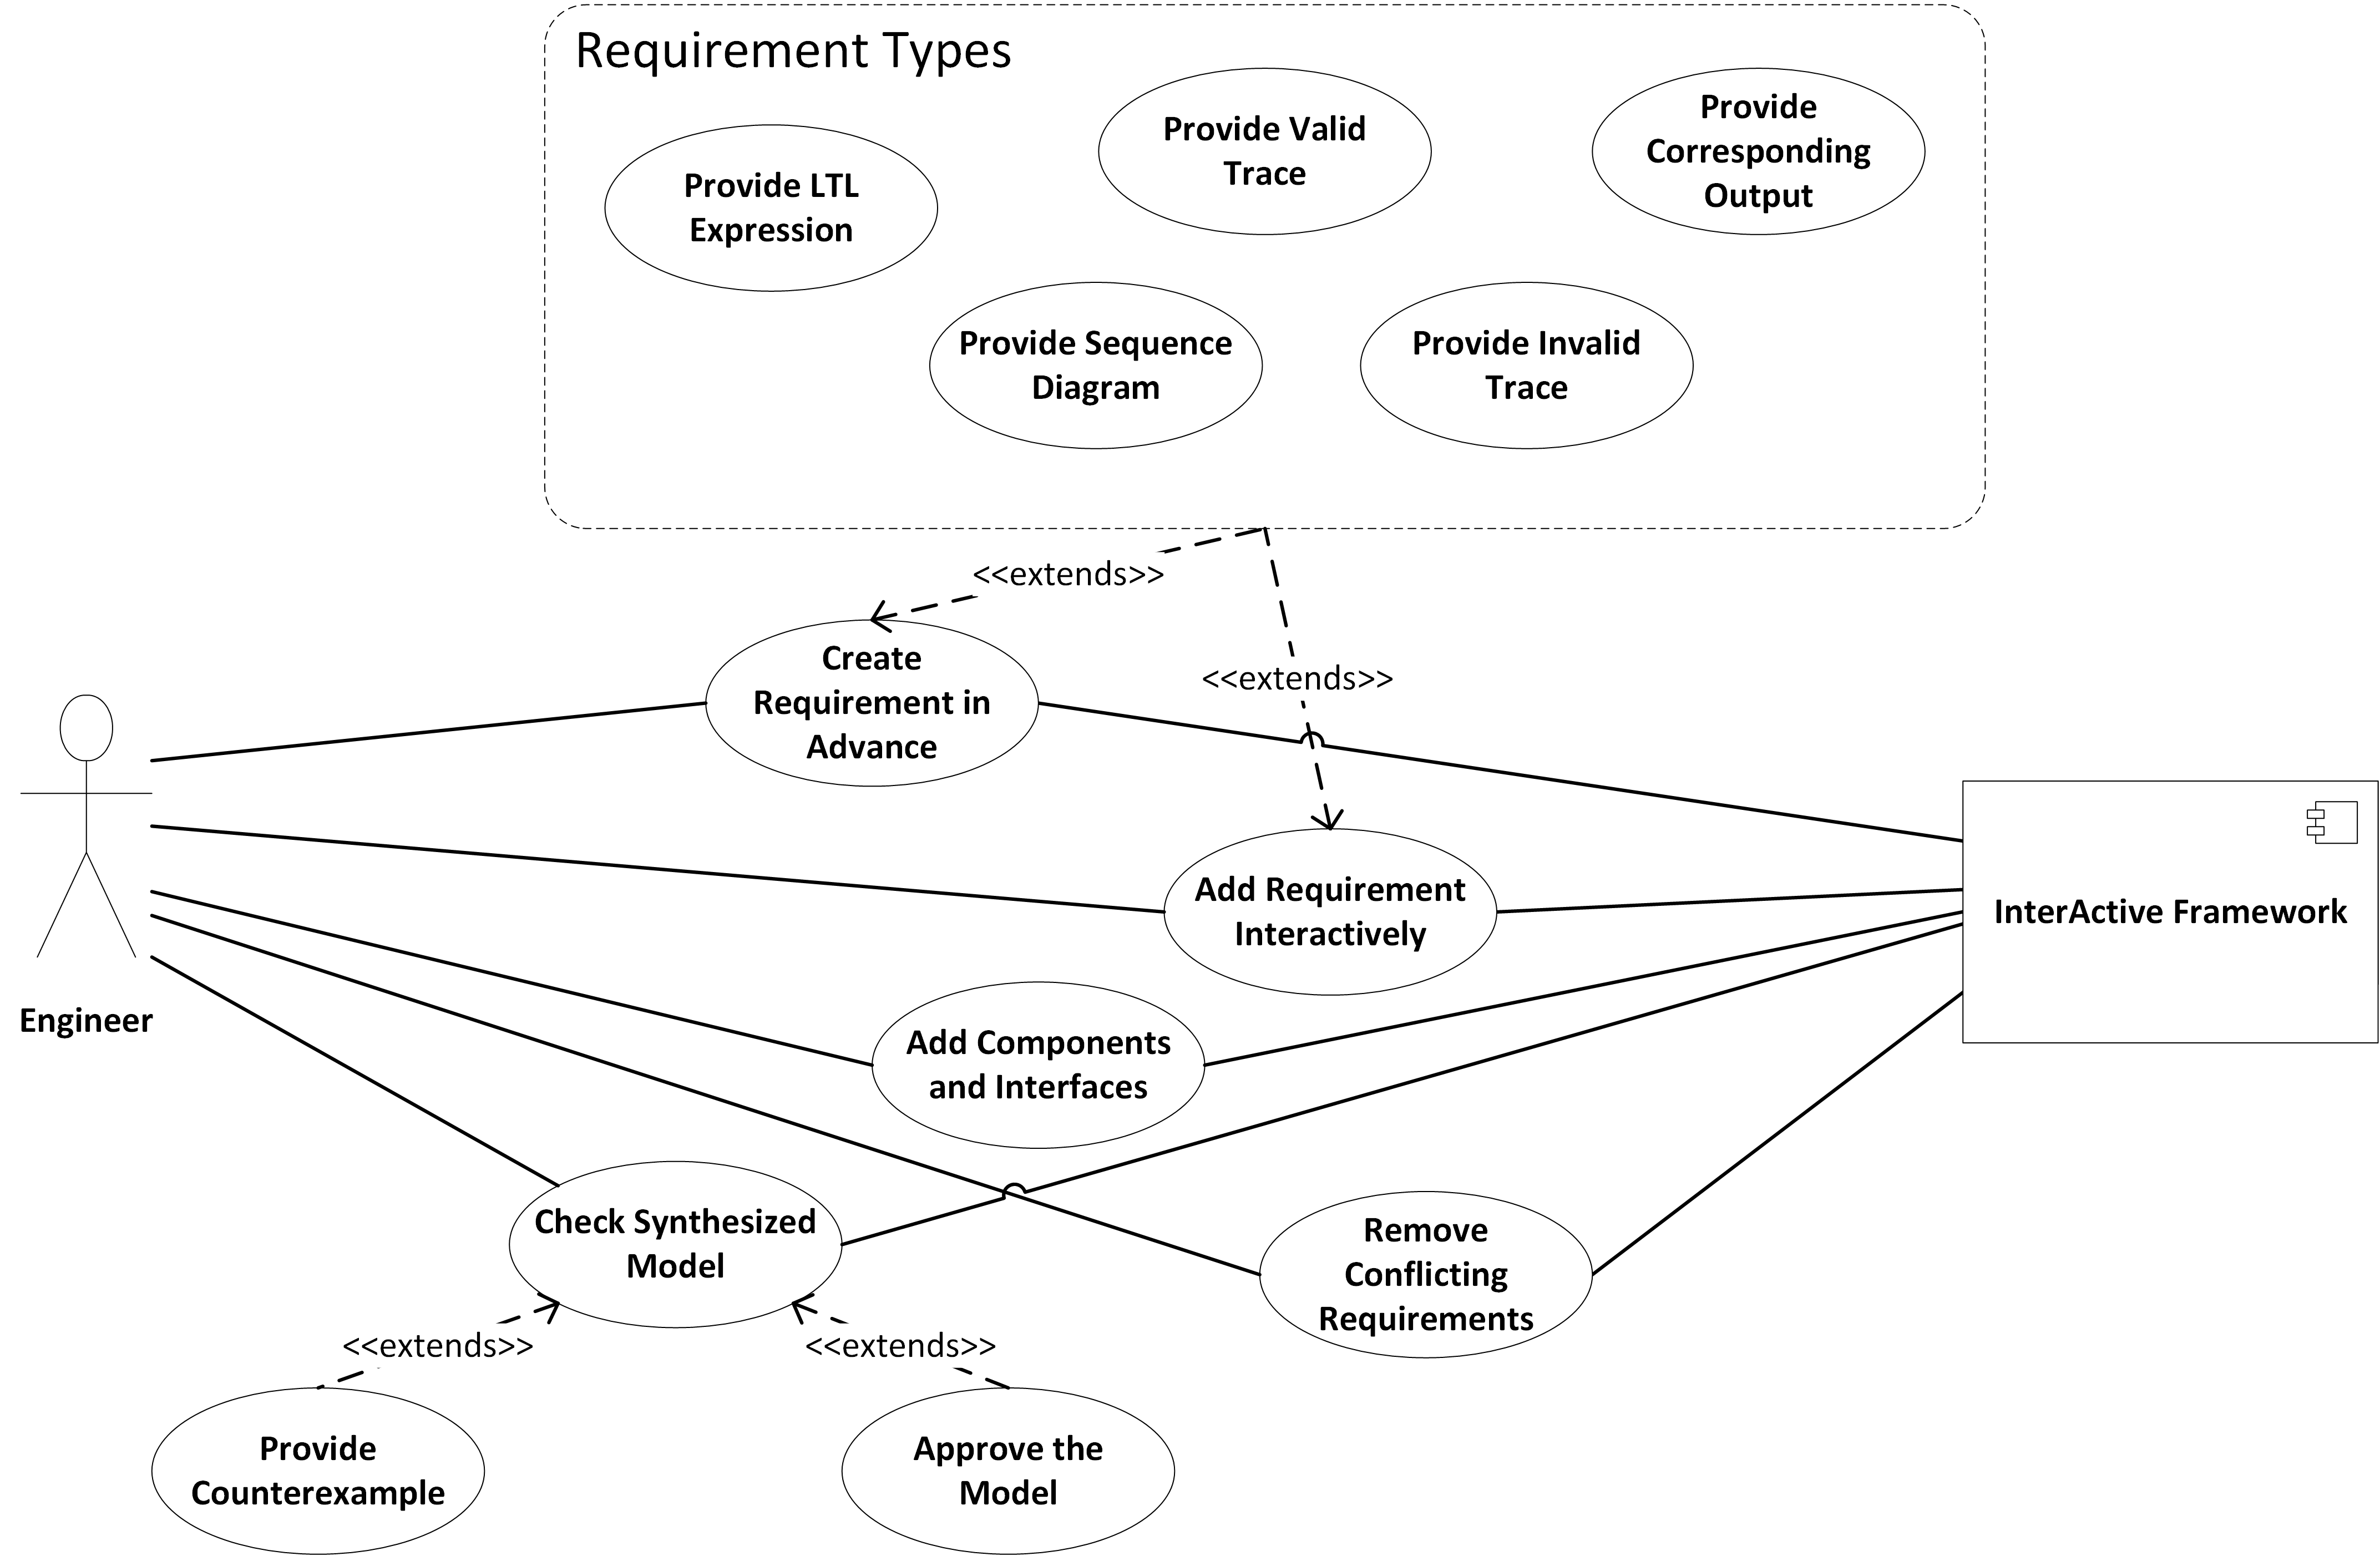
\includegraphics[width=150mm, keepaspectratio]{figures/methodology_interactiontypes.png}
	}
	\caption{Possibilities of the Engineer} %TODO title, extend 
	\label{fig_methodology_interactiontypes}
\end{figure}

Our methodology is heavily based on the interaction of the user with the system, especially its \textit{Oracle} component. The different types of interaciton are summarized on Figure \ref{fig_methodology_interactiontypes} and elaborated on in Subsection \ref{subs_reqtypes}. These interactions take place in a predefined order, illustrated on Figure [TODO] and have a predefined syntax with the corresponding semantics. Their common feature is the declarative way of describing the system components, which allows the engineer to focus solely on the expected behavior and acquire a minimal model exhibiting the specified functionality.

[TODO WORKFLOW KÉP IDE] %TODO

%---------------------------------------------------------------
\subsection{Component Definition} \label{subs_compdef}
%---------------------------------------------------------------
%TODO megadhat több komponenst, névvel, ezek a megfelelő viselkedéseket fogják tanúsítani. I/O ábécét megadjuk előre, komponensek kapcsolatát a nevekből inferáljuk. Mindegyiket TELJESEN KÜLÖN tanuljuk.

%---------------------------------------------------------------
\subsection{Requirement Types} \label{subs_reqtypes}
%---------------------------------------------------------------
%TODO kifejteni ami a use-case diagramon van egyesével.
%LTL-nél kifejteni a szintaxist, LTS szemanitikát
%Szekvencia???
%---------------------------------------------------------------
\subsection{Equivalence Query} \label{subs_eq}
%---------------------------------------------------------------
%TODO megjeleníti az EQt, ha nem tetszik, adjunk ellenpéldát.
%Ha tetszik, elfogadjuk és továbblép a kövi komponensre vagy szerializál
%---------------------------------------------------------------
\subsection{Output} \label{subs_resultingmodel}
%---------------------------------------------------------------
%TODO valid Gammát kapunk, ezt:
%kiegészíthetjük
%generálhatunk belőle akármit


%----------------------------------------------------------------------------
\section{Overview of the Architecture} \label{sec_architecture}
%----------------------------------------------------------------------------